% \textcolor{blue}{
% \textbf{Deliverables:}
% \begin{itemize}
% \item requirements $\xrightarrow{\rm status}$ draft
% \item concept design (if necessary baseline and backups) including 3D model
% \item main questions to answer in this subsection
%   \begin{itemize}
%   \item number of coils
%   \item coil size
%   \item power consumption
%   \item envelope for inductance
%   \item active component?
%   \item minimum number of magnetometers
%   \item achievable sampling frequency, ...
%   \end{itemize}
% \item calculations proving that the design concept fulfills the requirements 
% \item interface definitions (detailed)
% \item design and manufacturing plan
% \item schedule
% a\end{itemize}
% }
\subsection{Overview}
The location of the nEDM spectrometer in an accelerator facility necessitates a system to reduce influences of environmental magnetic fields on the experiment. As mentioned in an earlier section, there is a strong background field up to $350\,\mu$T in the TUCAN area in the TRIUMF Meson Hall. The FEA simulations revealed that such a strong field could saturate the mu-metal layers of MSR, and worsen its shielding performance (Sec. \ref{msr:FEA}). In addition, there are occasional field perturbations on the order of $\sim 10\,\mu$T, which may require idealization procedures of MSR. 

The Ambient Magnetic-field Compensation (AMC) subsystem will consist of a set of coils and magnetometers to provide static and dynamic magnetic field compensation in the exterior of MSR to ensure the shielding performance of MSR and increase possible uptime of the EDM measurements. This section specifies the key requirements of  AMC and summarizes developmental works performed in this context.  





\subsection{Purposes}

To understand the magnetic environment of the experiment and to clarify the requirements on the compensation system, typical numbers characterizing the environmental magnetic fields in the TUCAN area are listed in Table \ref{tab:amc_comparaion}, in comparison to those of the PSI nEDM experiment.
The values of PSI are based on preceding works on the corresponding system of the PSI experiment \cite{Afach2014}, which provides static and dynamic compensation of the magnetic field surrounding its mu-metal shield. In what follows, we discuss the motivations for the TUCAN AMC subsystem, highlighting differences from and similarities with the PSI environment.

One significant difference between the two is the order-of-magnitude stronger static background field in the TUCAN area which is due to the stray field of the TRIUMF cyclotron. Once this problem is dealt with and TUCAN MSR performs as its design, it is expected to suppression of the background fluctuations of $\lesssim 80\,$nT order (in the averaging time of $\sim 100\,$s) to a level of $\sim10\,$pT, sufficient for what is required for the EDM measurement [ref, earlier section]. Thus the dynamic compensation of field fluctuations is not required for TUCAN AMC to achieve required field stability as long as the functionality of MSR is ensured. However, there are occasions when we would need dynamic compensation of field variations, which we shall discuss next. 

Occasional magnetic field variations on the order of $\sim 10\,\mu$T exist in both cases. In the case of the PSI experiment, neighboring superconducting magnet test facilities were operated on a daily bases, producing magnetic field variations up to $30\,\mu$T. According to \cite{Afach2014}, the mu-metal shield needed to be idealized after experiencing such field variations. The needs of the idealization procedure, which typically took about 30\,min to an hour for each time, were reduced by the dynamic compensation suppressing them by a factor of $\approx10$ [Afach2014]. In the case of TUCAN, an overhead bridge crane in the hall, which is operated typically once in a few days, is found to produce magnetic field variations on a comparable order. Therefore we should anticipate that these field variations would require the idealization procedure. Active magnetic field compensation will possibly reduce the needs of idealization procedures. Further, if it can suppress some of the field variations to the order of $1\,\mu$T or below, it can even make the EDM measurement possible under such field variations.

Based on the above discussions, the goals of the AMC subsystem are summarized as below:
\begin{itemize}
  \item To provide static magnetic field compensation to prevent the background field of $\approx 350\,\mu$T from saturating MSR. 
  \item To provide dynamic compensation of magnetic field variations. Its main target is perturbations on the order of $\sim 10\,\mu$T. This will increase the potential uptime of the EDM measurements by reducing the needs of idealization procedures and suppressing the field variations to a level required for the measurements.
\end{itemize}

\begin{table}[tb!]
\centering 
\begin{tabular}{|l||c|c|}
\hline

 & \multicolumn{1}{c|}{\textbf{PSI}} & \multicolumn{1}{c|}{\textbf{TUCAN}} \\ \hline\hline 
Static background field & $\approx62\,\mu$T & $\approx 350\,\mu$T            \\ \hline
Background field fluctuations $\sigma_{|\mathbf{B}|}(100\,\mathrm{s})$ & $\approx 1\,\mathrm{nT}$ (night), $\approx 80\,\mathrm{nT}$ (day) & $\lesssim 80\,\mathrm{nT}$ \\ \hline
Occasional variations  & $\lesssim30\,\mu$T  & $\lesssim 10\,\mu$T      \\ \hline
 MSR shielding factor    &  $\sim 10^4$  &  $\sim 10^5$ (planned) \\ \hline 
\end{tabular}
\caption{List of typical numbers characterizing the magnetic field environment of the PSI nEDM experimental site and the TUCAN area in TRIUMF Meson Hall. The table consists of typical values of, the static background field, the magnetic field fluctuations evaluated by the Allan deviation with an averaging time of 100\,s, typical amplitudes of occasional magnetic field variations, the quasi-static shielding factor of MSR. The values of the PSI experiment are based on \cite{Afach2014,Fra:phd,baker2014apparatus}. Those of TUCAN are based on \cite{Sarte2013} and recent measurements discussed in Section \ref{sec:amc_recent}. 
}
\label{tab:amc_comparaion}
\end{table}


\subsection{Requirements}
The key requirements specifications on the performance of AMC are stated below:

\begin{RSenumerate}[resume]
\item  The static magnetic field compensation of AMC should reduce the field surrounding MSR such that $|\mathbf{B}|<0.1\,$T is satisfied in the mu-metal layers of MSR. \label{RS:amc_rs_sta}
\begin{itemize}
  \item[\textbf{Rationale:}] The saturation magnetic induction of mu-metal is about $ 0.7\,$T. We require $|\mathbf{B}|<0.1\,$T to have a large enough safety margin.
  \item[\textbf{Test:}] In defining the geometries of the coils, FEA simulations are essential which include a realistic background field, MSR, and the compensation coils to confirm that the requirement is satisfied. On-site tests should also be performed in the commissioning phase of AMC.
\end{itemize}

 \item The dynamic compensation of AMC should compensate the external field variations on the order of $\sim 10\,\mu$T by a factor of $\approx 10$ when they are experienced by MSR. \label{RS:amc_rs_dyn}
 \begin{itemize}
  \item[\textbf{Rationale:}] 
  There are not many preceding studies on the threshold above which a given magnetic shield needs idealization. However, the reduction by a factor $\sim 10$ would significantly lessen the influence of the perturbations to MSR. This is also a realistic aim, regarding the preceding work by the PSI nEDM \cite{Afach 2014}. 
  \item[\textbf{Test:}] 
  To achieve this, the spatial and time properties of the target magnetic field variations are important factors. The geometries of the coils should be designed to compensate them adequately.
\end{itemize}

 \item The target of the static and dynamic compensation of AMC should include a volume which contains the parts of MSR which are moved by opening or closing of the door of MSR \label{RS:amc_rs_volume} (See Fig.\,\ref{MSR:mesonhalltop}).
 \begin{itemize}
  \item[\textbf{Rationale:}] In order to prevent saturation of these parts. This will be required for operation as well as commissioning of MSR. 
  \item[\textbf{Test:}] Should be taken into account in the design and test processes described in \ref{RS:amc_rs_sta} and \ref{RS:amc_rs_dyn}.
\end{itemize}
\end{RSenumerate}

The AMC subsystem is still in the phase of conceptual design, therefore its hardware requirements have not been clarified yet. 
They should include, for example, space requirements in order not to interfere with the other subsystems, the response times of the system which would constrain the inductance of the coils and switching times of the power supplies, and an adequate rate and accuracy for the readout of the magnetometers. They will be detailed as the design work proceeds. 

\subsection{Developmental works for the design of the compensation system}

In the following, recent developmental works performed for the design of AMC are summarized. 

\subsubsection{Feasibility check of the static compensation}\label{sec:amc_feasibility}
\begin{figure}[htb]
  \centering
  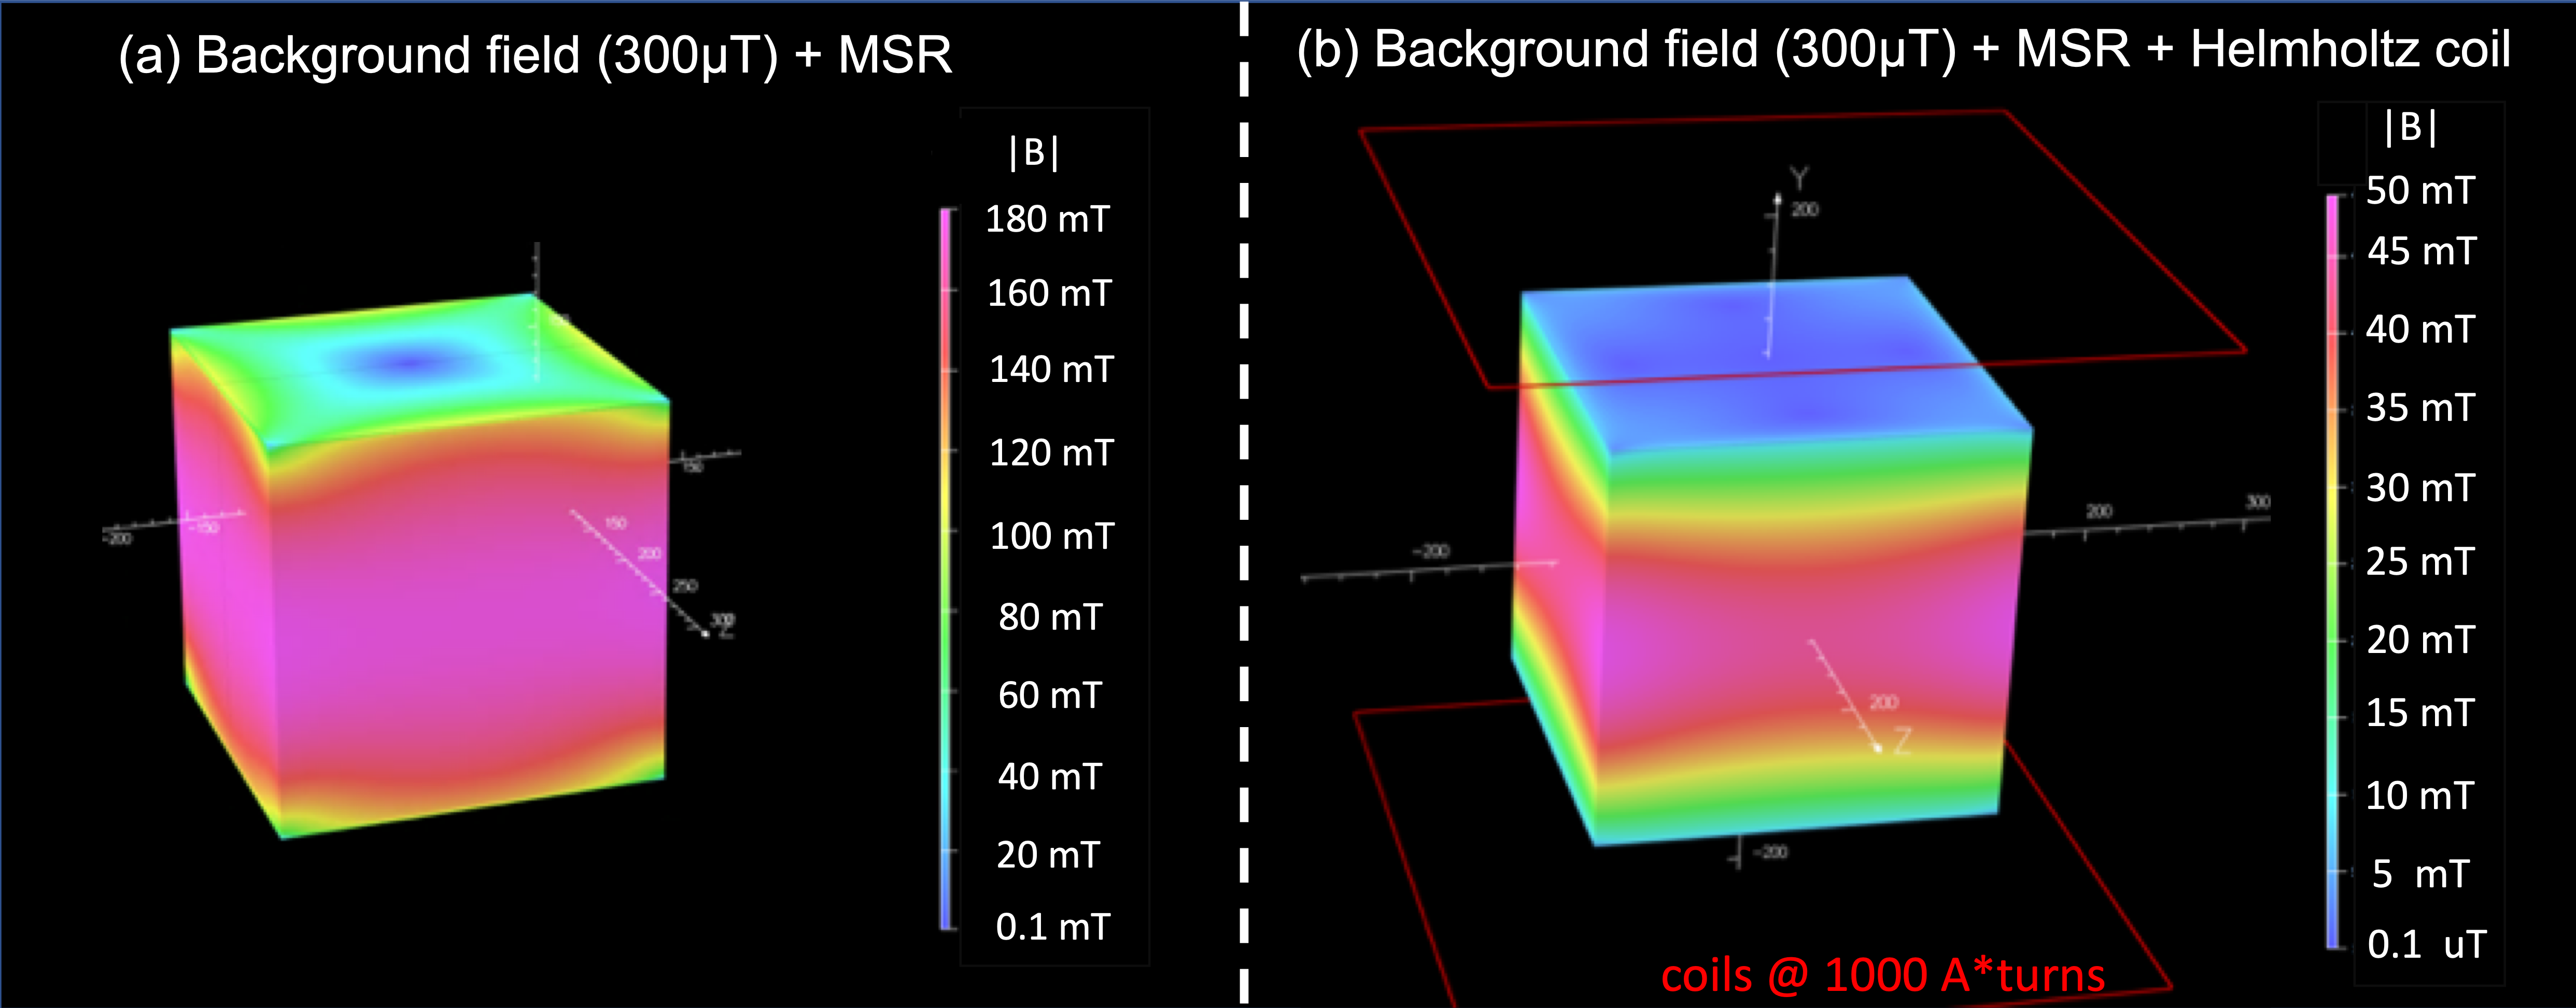
\includegraphics[width=\textwidth]{graphics/AMC/feasibility.png}
  \caption{FEA simulations to confirm the feasibility of the static compensation to prevent saturation of mu-metal layers of MSR. (a) A two-layer mu-metal box with the outer layer size of 2.34\,m x 2.34\,m x 2.34\,m is placed in a homogeneous background magnetic field. The background field has a strength of $300 \mu$T and directed along the vertical axis of the model. The field resulted in the outer mu-metal layer is at a maximum of $180\,$mT. (b) A Helmholtz coil pair (each coil with a size of 4\,m x 4\,m, placed apart by 3.8\,m) with 1000 A$\cdot$turns is added to the model of (a). It can be seen that the field in the outer mu-metal layer is reduced to $<50\,$mT.  }
  \label{fig:amc_feasibility}
\end{figure}
Shown in Fig.\,\ref{fig:amc_feasibility} are results of FEA simulations performed to confirm the feasibility of the static compensation of a background field on the order of $\sim 100\,\mu$T. In Fig.\,\ref{fig:amc_feasibility}\,(a), a two-layer cube of mu-metal representing MSR is placed in a homogeneous background field of $300\,\mu$T. The magnetic flux density $|\mathbf{B}|$ produced in the outer mu-metal layer of MSR is shown in the color scale. In the strongest area, the flux density goes up to 180\,mT. In Fig.\,\ref{fig:amc_feasibility}\,(b), a Helmholtz coil pair surrounding the cube is added. With current$\cdot$turns of 1000\,A$\cdot$turns on these coils, the flux density in the outer mu-metal layer is reduced to $<50$\,mT.

From this it seems feasible to reduce the influence of the background field of $100\,\mu$T order to the required level by coils with currents$\cdot$turns on the order of $\lesssim 1000\,\mathrm{A}\cdot$turns, In reality, the background field has an inhomogeneous spatial distribution, which should be taken into account in designing the actual system. 




\subsubsection{Recent magnetic field measurements in Meson Hall}\label{sec:amc_recent}
\paragraph*{Measurement setup}
Characterization of the on-site magnetic fields is essential for proceeding in the design of the AMC coil system. To acquire necessary data, a series of measurements were performed in the TUCAN area in the summer of 2019. The rest of this section gives a summary of these measurements.

The measurement campaign was performed for three purposes below :
\begin{itemize}
  \item Characterization of the static background field around the planned volume of MSR
  \item Characterization of magnetic field variations produced by motions of the overhead bridge crane
    \item Evaluation of typical background magnetic field fluctuations in the TUCAN area.
\end{itemize}
The layout of the measurements is shown in Fig.\,\ref{fig:amc_layout}. The coordinate system $(x,y,z)$ was defined to be used throughout the measurement campaign. 
For the characterization of the background field, the grid with 40\,cm intervals is defined as shown in the figure. The field in this volume was mapped by translating the position of a triaxial fluxgate magnetometer over the grid. The mapped volume had a maximum height of 3.89\,m from the floor and thus contained about 74\% of the planned volume of MSR. 
 \begin{figure}[htb!]
   \centering
   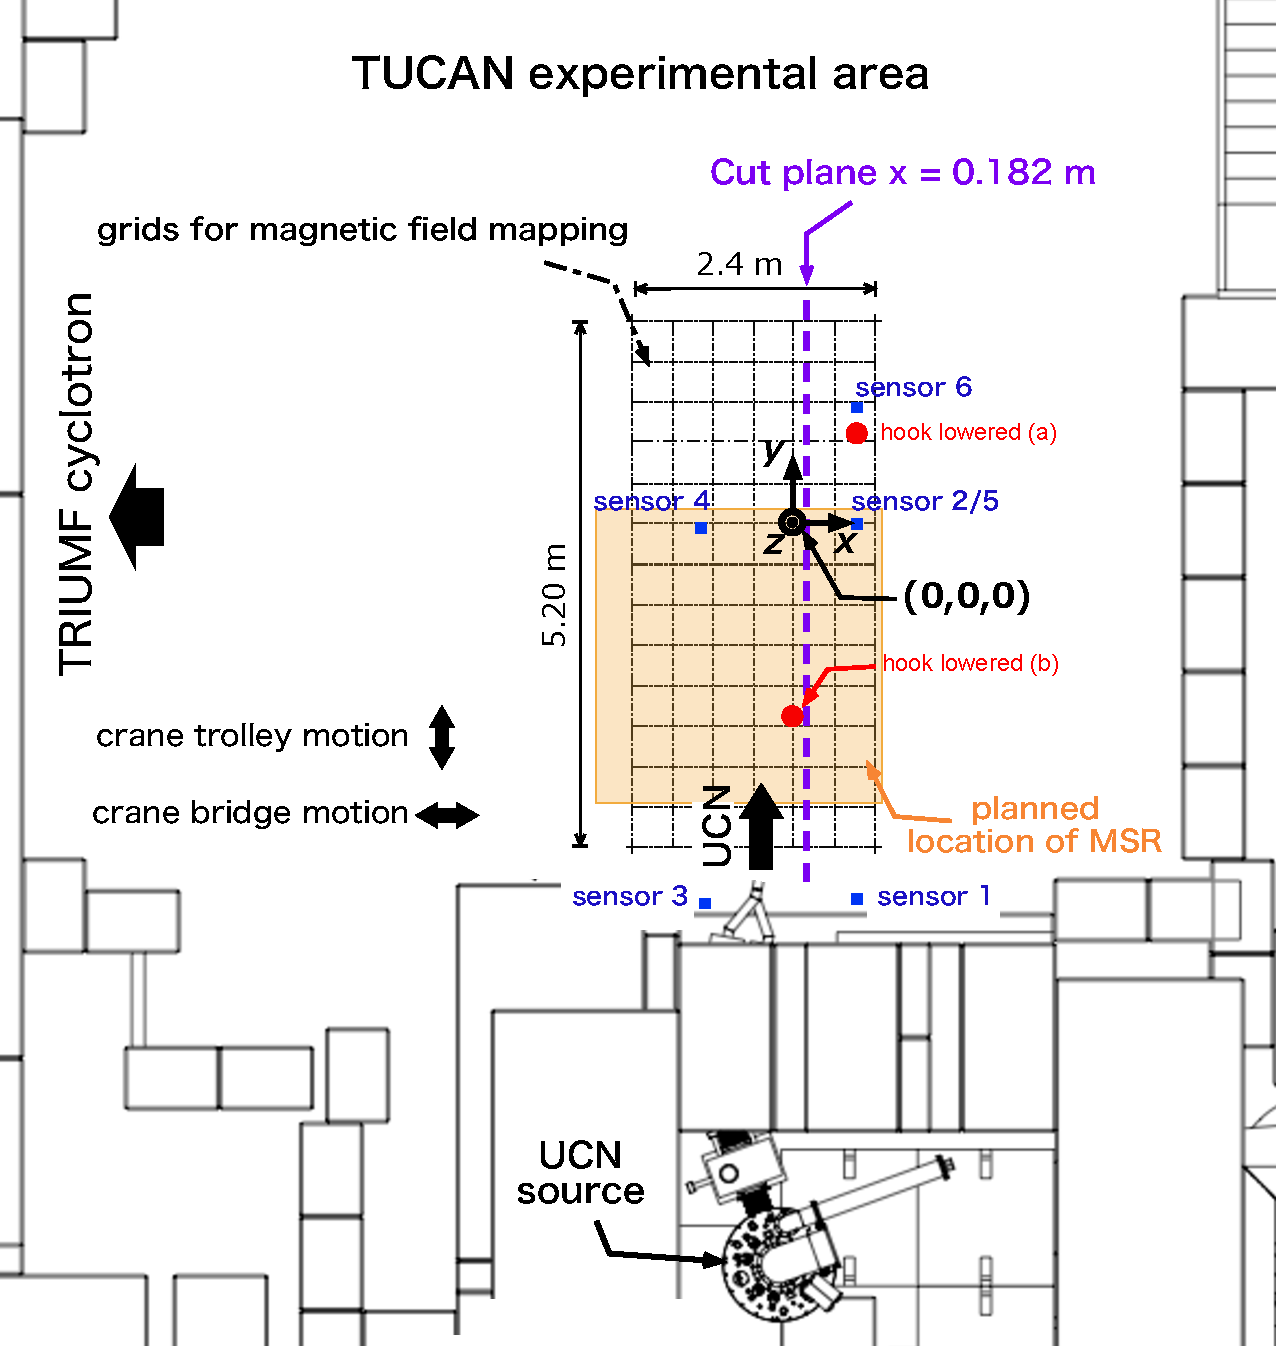
\includegraphics[width=.9\textwidth]{graphics/AMC/Layout_CDR.pdf}
   \caption{Layout of Meson Hall during magnetic field measurement campaign in the summer 2019. The coordinate system of the measurements $(x,y,z)$ is defined as shown ($z=0$ corresponds to the floor level).
   The grid with an interval of 40\,cm spanning over a volume of about 2.4\,m x 5.2\,m x 3.9\,m, containing the planned location of MSR is defined to map the static background field. The blue squares are the positions of six triaxial fluxgate sensors placed to characterize the magnetic field variations produced by motions of the overhead bridge crane. The height of the sensors is $z=0.402$\,m for sensor 5, and $z=1.417$\,m for the rest. During this test, the hook of the crane was lowered to characterize the field produced. The two spots where the hook was lowered are indicated by the red circles in the layout.
   The black arrows indicate the direction of the TRIUMF cyclotron, directions of two motions of the overhead bridge crane in the hall, the direction of UCN extraction from the source to the experimental area. }
   \label{fig:amc_layout}
 \end{figure}
 The sensors 1--6 in Fig.\,\ref{fig:amc_layout} indicate the positions of the fluxgate magnetometers placed to characterize the field variations caused by the crane motions. 
% To characterize the field variations caused by the crane motions, six triaxial fluxgate magnetometers were placed at positions indicated by the blue squares in the layout of Fig.\,\ref{fig:amc_layout}. 
%They measured the magnetic field while the crane was operated above the area.  
Each of the three possible patterns of motions of the crane: the bridge motions, the bridge motions and lowering and raising the hook, were tested\footnote{For the definition of the parts \textit{bridge} and \textit{trolley} of a bridge crane and their motions, see, for example, \url{https://www.gruasyaparejos.com/en/overhead-crane/}. The directions of the bridge- and the trolley motions of the crane in Meson Hall are indicated by the black arrows in Fig.\,\ref{fig:amc_layout}.}: 
The hook was lowered and then raised at two spots in the area. Their approximate positions marked by the red circles in the layout. 

The background magnetic field fluctuations in Meson Hall were evaluated from data of a triaxial fluxgate magnetometer placed at a fixed location $(x,y,z) \approx (-0.2\,\mathrm{m}, -2.0\,\mathrm{m}, 2.98\,\mathrm{m})$ marked by the green 'x' in Fig.\,\ref{fig:amc_layout}.




\paragraph*{Characteristics of the static background field}
Fig.\,\ref{fig:amc_B-map_cut} and \ref{fig:amc_B-map_3D} show the maps of the 
static background field obtained by the measurement. Fig.\,\ref{fig:amc_B-map_cut} shows a two-dimensional cut view of three-dimensional maps at a plane $x=0.182\,\mathrm{m}$. Some observations which can be made from these results are 
\begin{itemize}

\item The field is about $|\mathbf{B}|\approx 350\,\mu$T in the strongest areas.
\item The spatial property of the field can be understood as a combination of the cyclotron stray field and local fields from the floor. At the height of $z \gtrsim 1.5\,\mathrm{m} $, the contribution from the cyclotron field is dominant, where each of the field components can be expressed as a smooth function of the position. The localities observed near the floor are likely due to magnetized steel reinforcement bars underneath the concrete floor.  
\item At height $z>1.5\,\mathrm{m}$, the dominant field component is the $z$ component $B_{z}\approx -240\mu$T, pointing downward.

\end{itemize}

\begin{figure}[htb!]
  \centering
  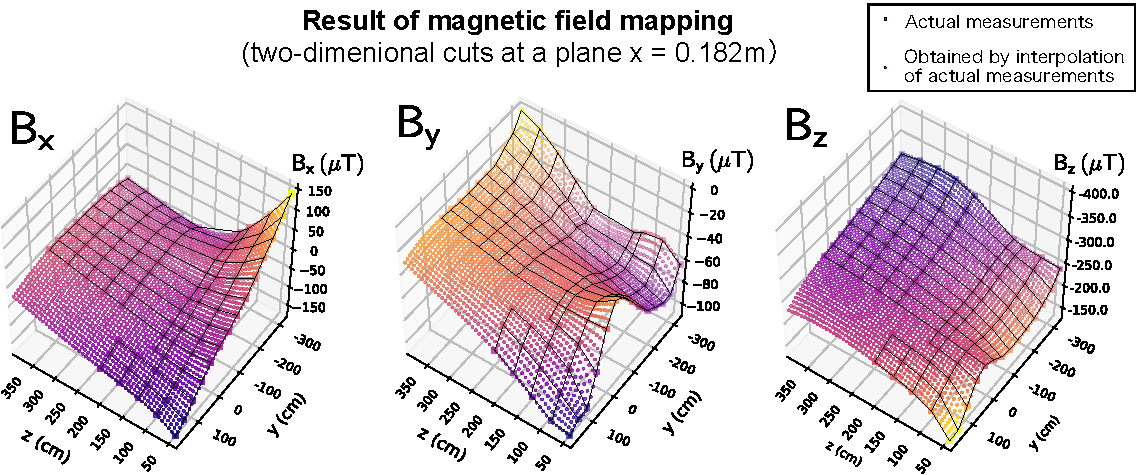
\includegraphics[width=\textwidth]{graphics/AMC/B-field_cut_CDR.pdf}
  \caption{Results of the mapping of the static background field. A two-dimensional cut of the three-dimensional map of the field $(B_{x}, B_{y}, B_{z})$ at a cut plane $x=0.182\,\mathrm{m}$ is shown. The square markers represent the data acquired by the actual measurements, and the circle dots show data obtained by interpolating the measured data points.}
  \label{fig:amc_B-map_cut}
  \vspace{1.5em}
  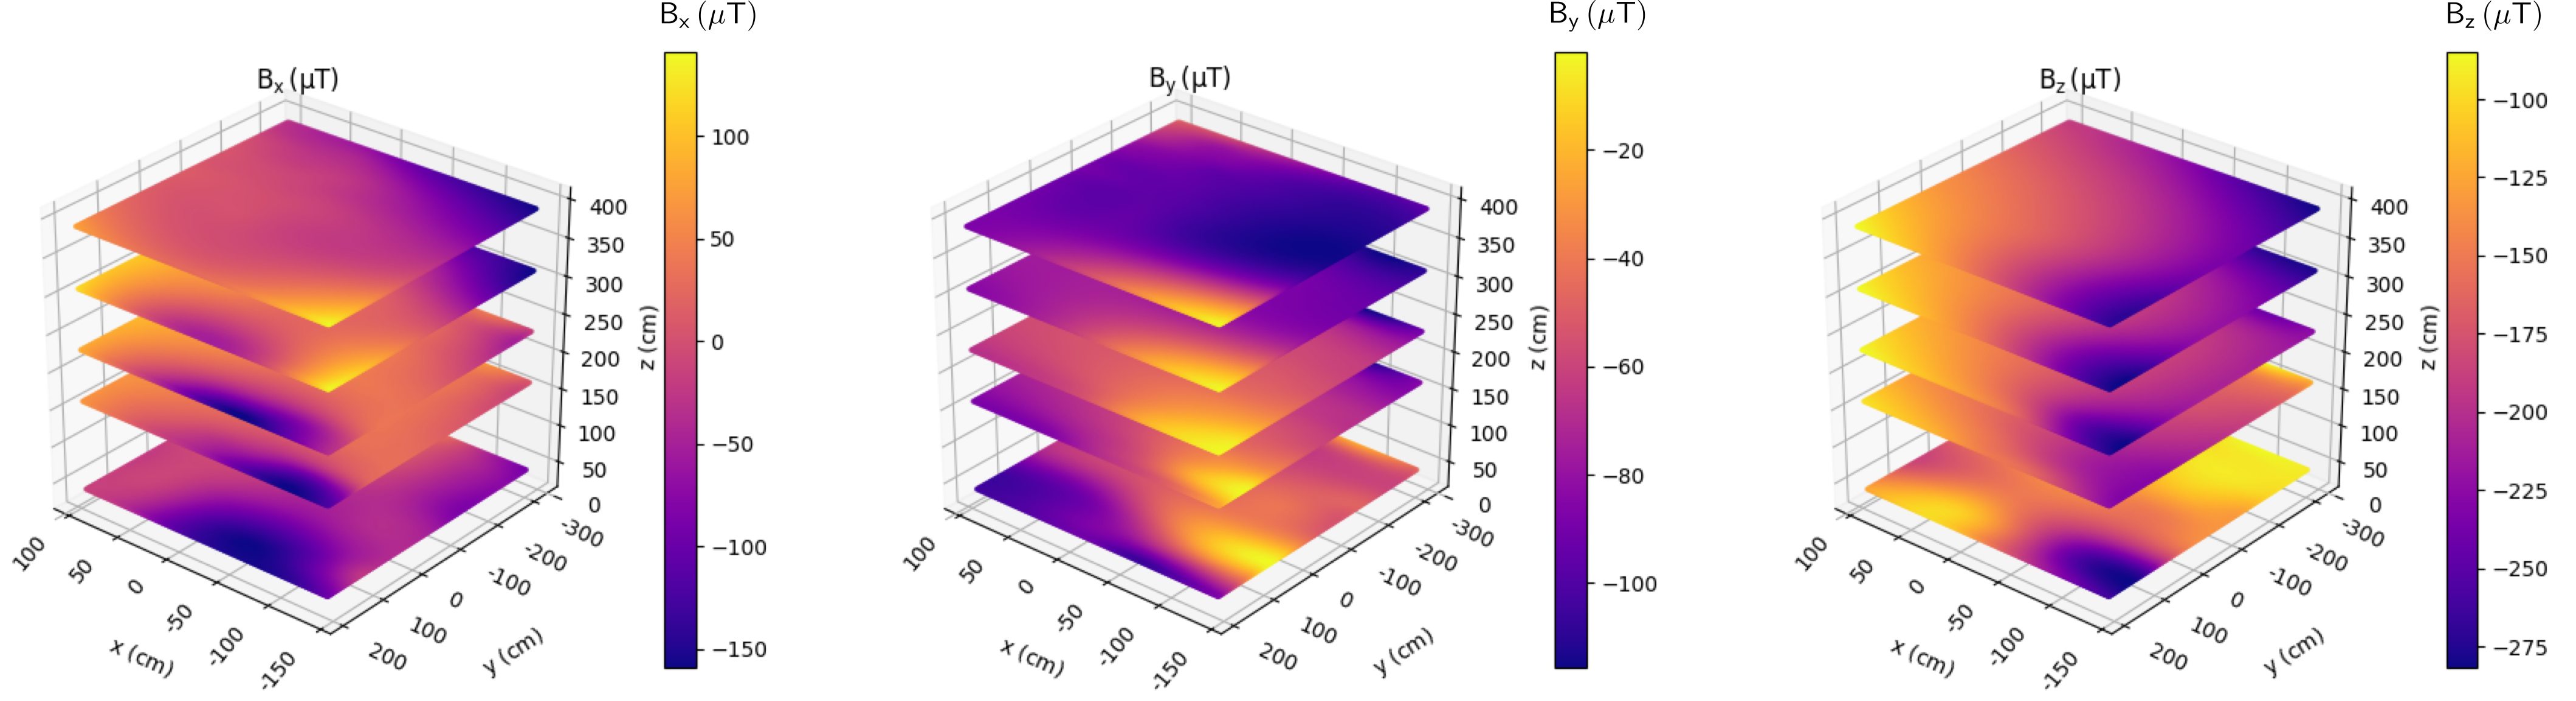
\includegraphics[width=1.02\textwidth]{graphics/AMC/B-field_3D.png}
  \caption{Three-dimensional color plots of each component of the static background field $(B_{x}, B_{y}, B_{z})$. The field component at each point is expressed in the color scale. The interpolation as shown in Fig.\,\ref{fig:amc_B-map_cut} is used to estimate field at positions in between points measured in the actual measurements. }
  \label{fig:amc_B-map_3D}
\end{figure}


\paragraph*{Characteristics of the field variations caused by the overhead crane}
To characterize the field variations induced by motions of the overhead crane, the field was monitored at the sensors at the six positions indicated in Fig.\,\ref{fig:amc_layout} while the crane was being operated.  
In Fig.\,\ref{fig:amc_crane}, the magnetic field measured by the six fluxgate sensors during the test is shown as a function of time. The offset of each sensor readout at the beginning of the test is subtracted to show the relative field variations. Some of the crane operations and positions are annotated on the figure. 

 First, the bridge of the crane was moved in $\pm x$ direction. Next, the trolley of the crane was moved in $\pm y$ direction while the bridge was parked above the TUCAN area. Lastly, to evaluate the influence of the hook of the crane, the hook was lowered and then raised. It was done at the two locations indicated by the red circles in Fig.\,\ref{fig:amc_layout}, first at  location (A), then at  location (B). 

To summarize the major features of the crane-induced field variations,
\begin{itemize}
\item The maximum field variations observed were about $\Delta B_{x}\approx -250\,\mu$T on sensor 6 when the hook was lowered in a neighborhood of the sensor at a distance of $\approx 30\,$cm. This is not of much concern in view of actual operations of MSR and AMC, because the operation of the hook would take place only in the maintenance period of TUCAN. It can also be found that the effects of the hook are highly local; e.g. for the hook motions at location (A), the variations are reduced to $<\left|30\,\mu\mathrm{T}\right|$ for each component when they were experienced by sensor 2, which was placed away from the hook location by $\approx 80\,$cm.
\item The trolley motions were found to produce much smaller variations than the bridge motions and were $<|1\,\mu\mathrm{T}|$ for each component. 
\item What matters the most among the three types of motions is the bridge motions along the $x$ axis. The zoomed-in plots in this time window are shown in Fig.\,\ref{fig:amc_crane}\,(b). The locations of the bridge at different times are annotated in the boxes in the figure. It can be seen that the field variations produced by different positions of the bridge are reasonably reproducible, and add $\Delta \mathbf{B}\approx (+6\,\mu\mathrm{T}, 0\,\mu\mathrm{T},+2\,\mu\mathrm{T})$ when the bridge is right above the TUCAN area. The variations are also rather homogeneous. Their inhomogeneities are evaluated to be $\Delta B_{i}/\Delta x_{j} < \left|2 \mu \mathrm{T}/ \mathrm{m}\right|$ (for $B_{i}= \{B_{x}, B_{y}, B_{z}\}, x_{j}=\{x,y,z\})$.
\end{itemize}

\begin{figure}[htbp!]
\centering
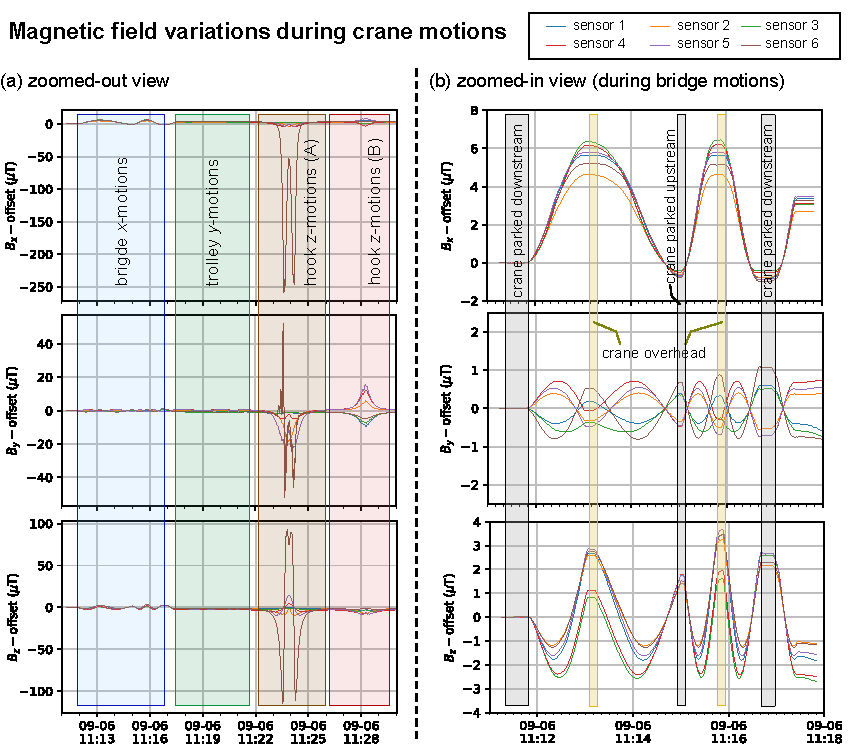
\includegraphics[width=\textwidth]{graphics/AMC/crane_test.pdf}
\caption{Characterization of magnetic field variations caused by the crane motions. The variations of the field were monitored by the six triaxial fluxgate magnetometers whose positions shown in Fig.\,\ref{fig:amc_layout}. The offset of each sensor reading at the beginning of the test is subtracted to show the relative field variations at each location. 
(a) The annotated boxes indicate the type of crane motions tested at each time window. The bridge motions in $\pm x$ direction, the trolley motions in $\pm y$ direction, and vertical hook motions were tested at location (A) and then at (B) (see Fig.\,\ref{fig:amc_layout}) were tested. (b) The zoomed-in plots in the time window of the bridge motions. Before starting the test, the crane was parked at a downstream ($+x$)  adjacent area of TUCAN. The crane passed over the area and parked a upstream ($-x$) area of TUCAN (see Fig.\,\ref{fig:amc_layout}).
} 
\label{fig:amc_crane}
\end{figure}
%\begin{table}[tb]
%\centering
%\caption{Parameters characterizing the magnetic environment of the TUCAN apparatus in the TRIUMF Meson Hall, listed in comparison of those of PSI-nEDM experiment. [Afash]
%Magnetic field environment in TRIUMF Meson Hall in comparison to PSI-nEDM experiment. }\label{tab:MSR-comparison}
%\vspace{1em}
%\begin{tabular}{|l|c|c|}
%\hline
% & TUCAN & PSI-nEDM \\ \hline \hline 
%Static background field strength $ |B|$ & $\approx 350\,\mu$T & $\approx 62\,\mu$T \\ \hline
%Fluctuations (@100\,s averaging) & $ \lesssim 100$\,nT & $\sim100\,$nT \\ \hline
%Occasional variations & $ \lesssim 30\,\mu$T (crane) & $ \lesssim 30\,\mu$T   (SULTAN/EDIPO)  \\ \hline
%MSR quasi-static shielding factor & $\sim 10^5$ & $\sim 10^4$ \\ \hline 
%\end{tabular}
%\end{table}

\paragraph*{Characterization of background magnetic field fluctuations}
Among the sensors shown in \ref{fig:amc_layout}, sensors 1--5 were fixed on the same locations since September 2019. The magnetic field in the area has been monitored by these five sensors for a few months with a constant sampling rate of 1 Hz\footnote{The raw data sampling rate was set to be 200 Hz in order to eliminate high-frequency noise. Every second, the sensor data acquisition  system averages 200 measurements to obtain one data point.   }. 
Typical magnetic field fluctuations were evaluated from this data in a time window of 2019-11-16 11:00--2019-12-15 20:00. Shown in \ref{fig:amc_stability-overview,fig:amc_stability-day-night} are results of the evaluation for data from sensor 4. 

(More explanations of the figures will be added by Monday ... )

Typical magnetic field fluctuations in Meson Hall was evaluated using 
\begin{figure}[htbp]
\centering 
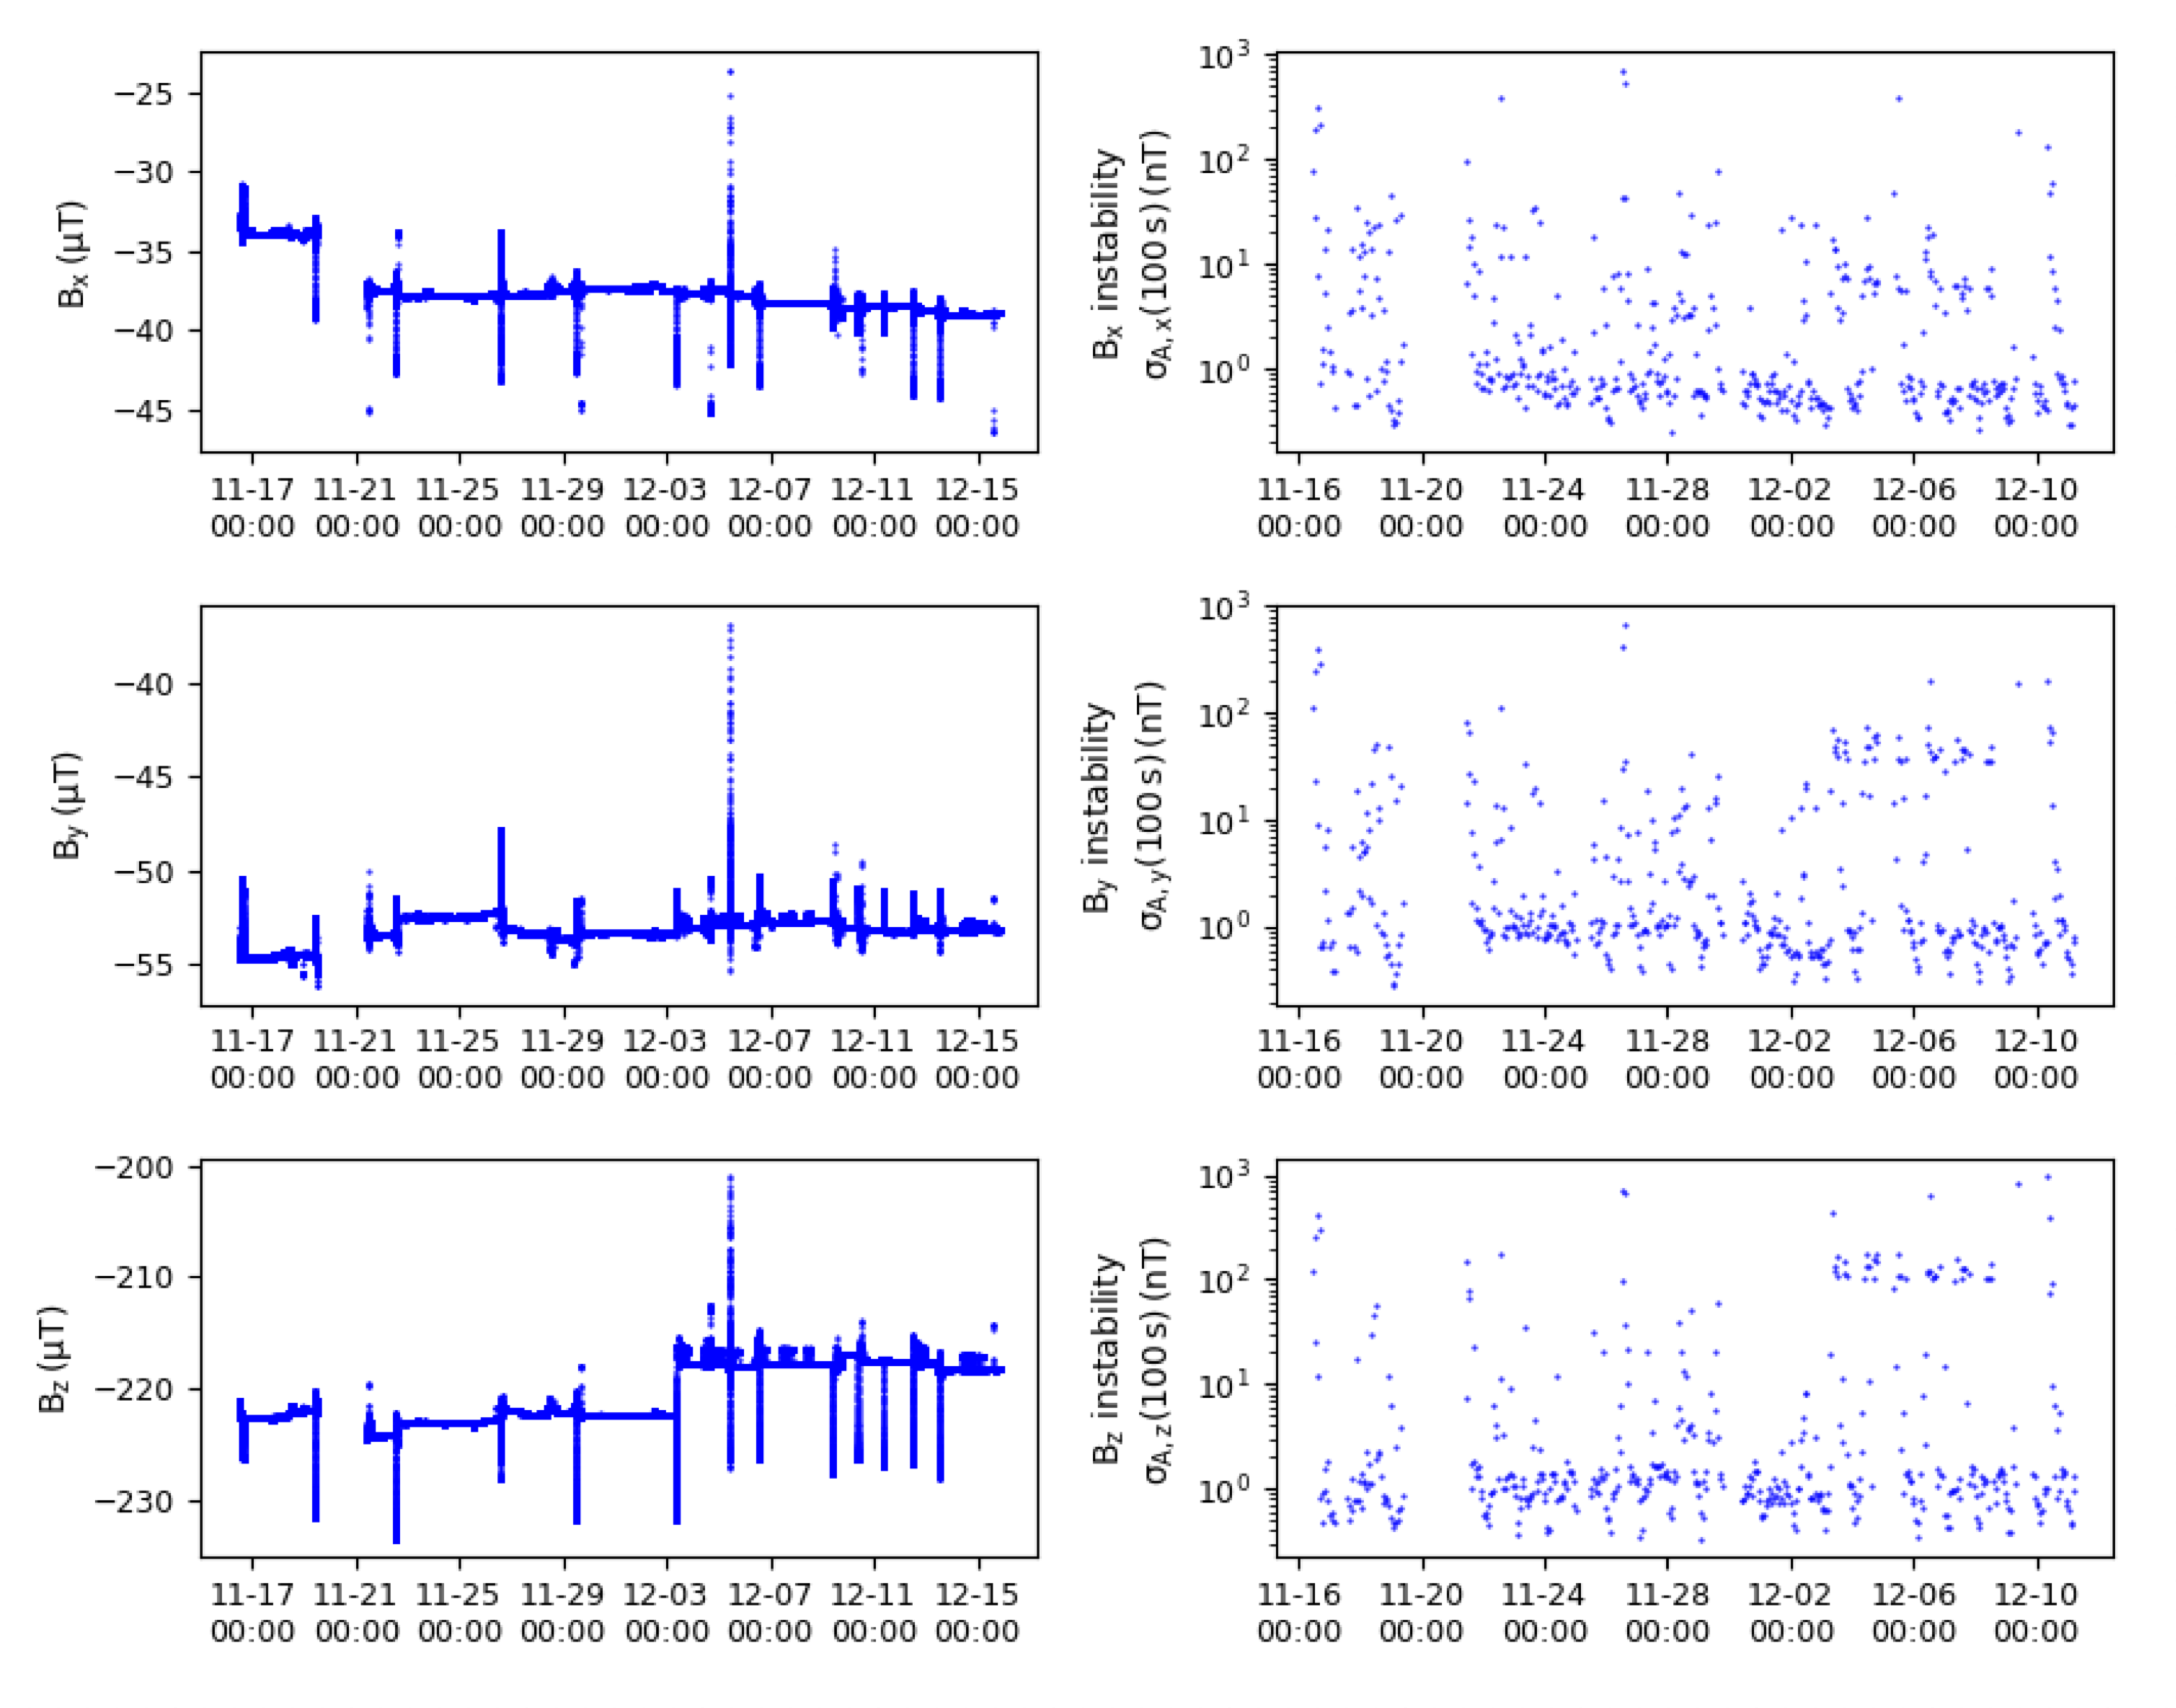
\includegraphics[width=.8\textwidth]{graphics/AMC/stability_overview.png}
\caption{default}
\label{fig:amc_stability-overview}
\end{figure}

\begin{figure}[htbp]
\centering 
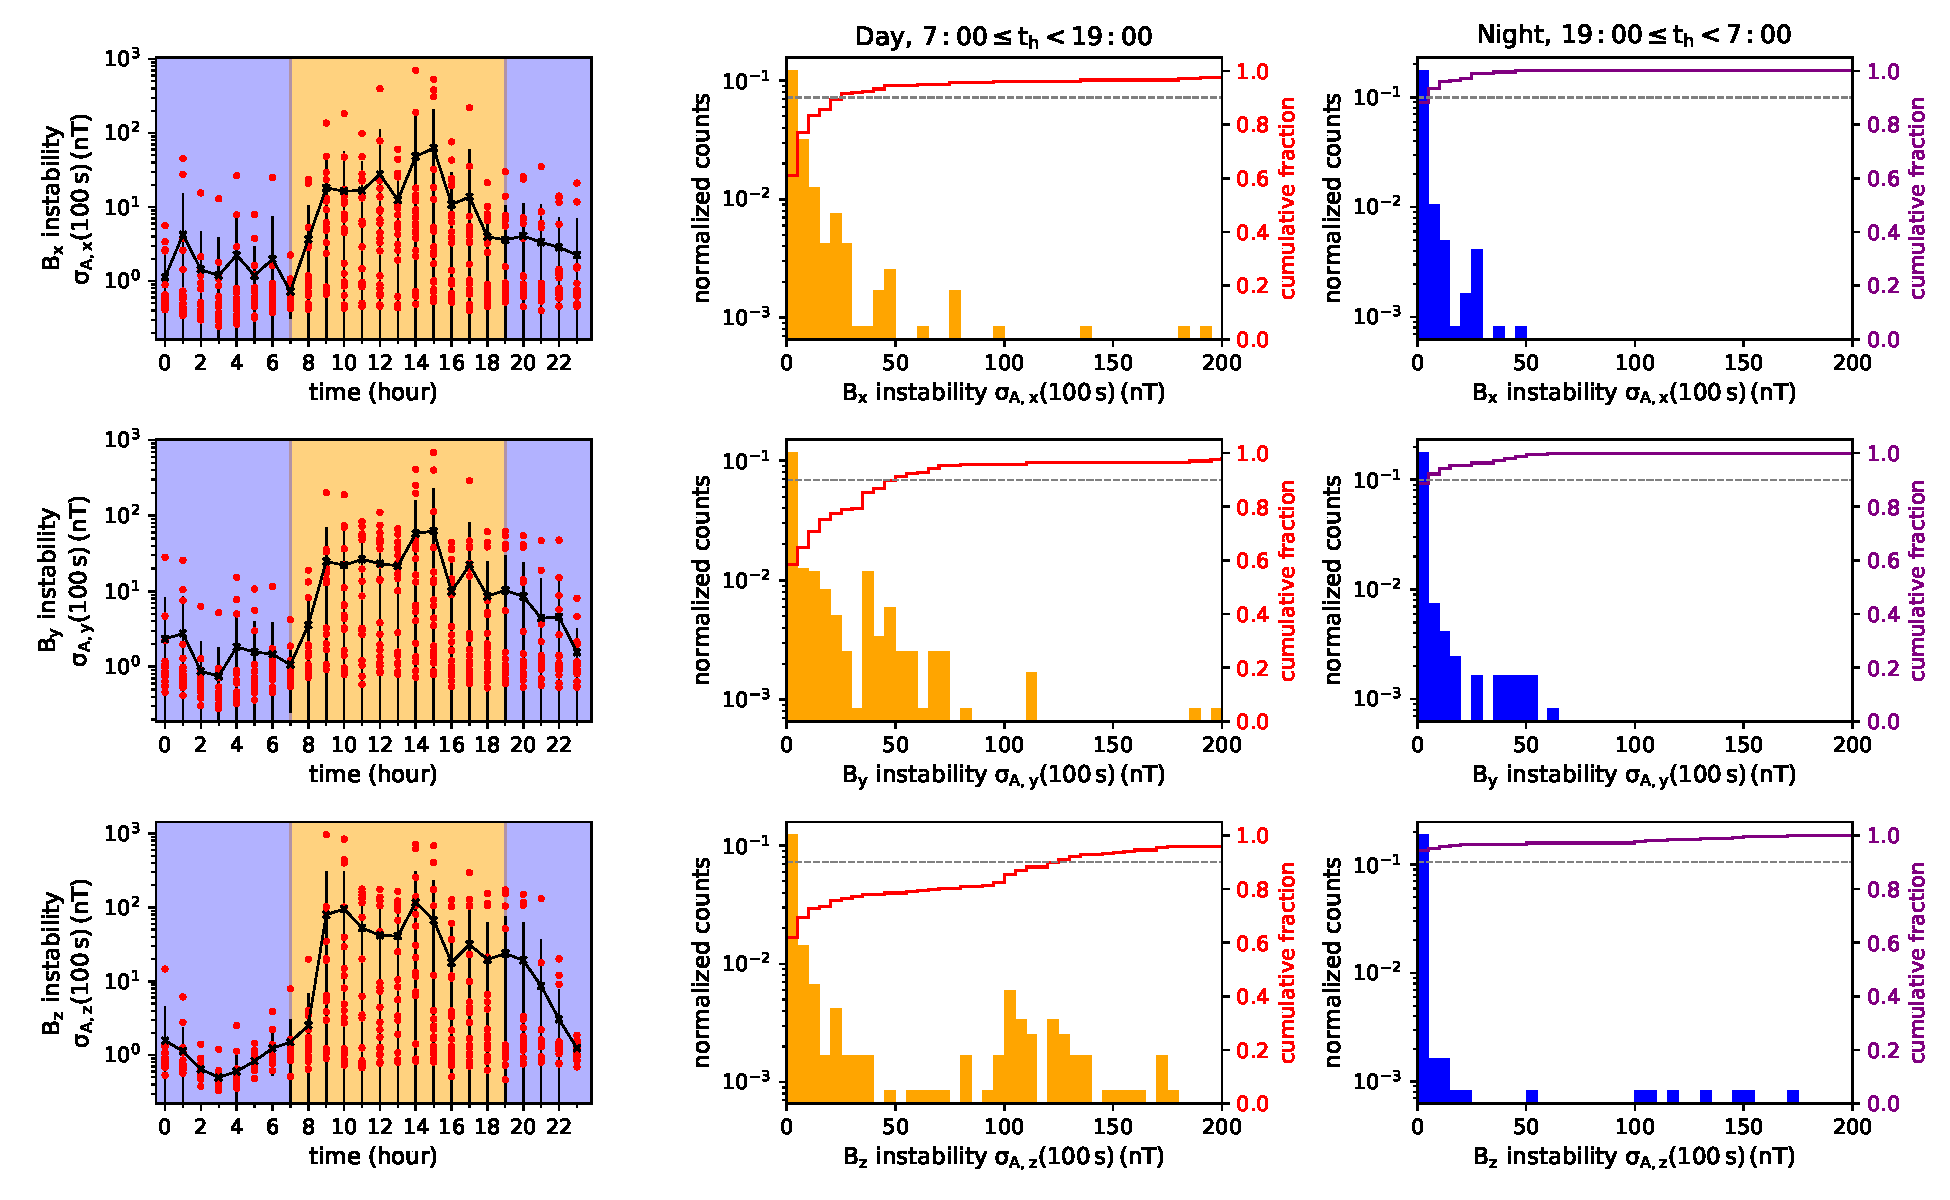
\includegraphics[width=.9\textwidth]{graphics/AMC/stability_day_night_f3_100s.pdf}
\caption{default}
\label{fig:amc_stability-day-night}
\end{figure}


%\begin{table}[tb!]
%\centering 
%\begin{tabular}{|l||r|r|r|}
%\hline
%
% \multicolumn{1}{|c||}{Time window}  & \multicolumn{1}{c|}{$\sigma_{A,x}(100\,\mathrm{s})$\,(nT)}& \multicolumn{1}{c|}{$\sigma_{A,y}(100\,\mathrm{s})$\,(nT) } &
%\multicolumn{1}{c|}{$\sigma_{A,z}(100\,\mathrm{s})$\,(nT) }\\ \hline \hline 
%(i) & 1.0\,(1) & 1.2\,(1) & 1.4\,(2) \\ 
%(ii) & 22\,(3) & 50\,(6) & 66\,(8) \\
%(iii) & 18\,(2) & 39\,(5) & 70\,(8) \\
%(iv) & 35\,(5) & 58\,(9) & 18\,(3) \\ 
%\hline 
%\end{tabular}
%\caption{
%}
%\label{tab:amc_datasets}
%\end{table}





\subsection{Timeline}
As of December 2019, the AMC subsystem is still in the phase of conceptual design. To decide on the geometries of the coils for static and dynamic field compensations, the following studies are underway:
\begin{itemize}
\item Search of optimum coil geometries that compensate for the measured magnetic field map.
\item Implementation of the spatial distribution of the measured field map in Opera-3D. This will be done by finding a magnetic scalar potential which produces the measured map with enough precision, by decomposition of the map with Legendre polynomials. 
\end{itemize}
We aim to complete these studies by the end of March, then the hardware design and development can be started.


% \subsection{DAQ/AMC Interface Requirements}

% Q1: Will your subsystem be providing a data stream (over some network connection) to the DAQ/controls? Or will you be providing an analog signal(s) that you want digitized by some DAQ/controls module? 
% If you are providing only a data stream, then you can skip question 2.

% A1: The AMC will provide a data stream


% Q3: Does your subsystem require a digitizer that is referenced to a central atomic clock?

% A3: No. The subsystem acquires magnetic field data and makes a response to it of necessity, but it is not required to synchronize this process to an external clock with extreme precision. The status of the system, such as recorded magnetic fields or currents set to coils will be recorded to MIDAS as for the other subsystems, but moderate precision of the absolute time is sufficient for this purpose, too.

% Q4: Does your subsystem have controls or gas handling like equipment?


% Q4.1 If yes does your equipment require PLC-type interlocks to ensure correct/reliable operation? Ie is there equipment-protection, safety or operational reasons why controls needs to be done with a PLC-type system? Or is it sufficient to have a computer program doing the control?

% A4: The control of the subsystem can be decided later, but seems to be ideal to use EPICS/MIDAS as for the other parts of the experiment. No gas handling like equipment is planned to be included in this subsystem.

% \begin{thebibliography}{9}
% \bibitem{Afach2015}
% Afach 2015

% \end{thebibliography}


% \begin{center}
% \textcolor{blue}{
% ------------------------------[Old draft ]--------------------------------------------
% }
% \end{center}







% \paragraph*{RS 3.-34}	The AMC shall reduce the external magnetic field to a level comparable to Earth magnetic field, less than 50 muT 
% \newline Rationale: 	
% %The passive shielding of the MSR can only handle a field of a certain magnitude, so the external field must be compensated.
% We do not expect the outer layer of the MSR to saturate (refer to A Sher's calculations to be inserted into this document), however, the manufacturer of the MSR will not certify it's a performance for any external field value larger than Earth field
% \newline Rationale: 	The 50 muT requirement is Earth’s field, but a smaller target field may be desirable
% \paragraph*{RS 3.-35}	The AMC shall be constructed in such a way that it does not prevent access to the MSR. A 'door', as well as a roof lid, might be required in the AMC coil cage.
% \newline Rationale: 	It will certainly be necessary to enter the MSR throughout the experimental run, so the AMC cannot render this impossible.
% \paragraph*{RS 3.-36}	The ambient field of the experimental area shall be mapped and monitored to a precision acceptable to specify the construction of the AMC; 
% \newline Rationale: 	It is important to understand the ambient magnetic conditions due to other magnetic equipment prior to running the experiment. ie the maximum DC values and amplitude of AC changes need to be known such that the right power and bandwith/speed of power supplies, as well as inductance of coils, can be chosen/determined.
% \paragraph*{RS 3.-37}	The ambient magnetic field control system shall be developed such that its cost falls within the CFI budget allocation.
% \newline Rationale: 	 This is necessary for completion of the experiment.
% \paragraph*{RS 3.-38}	Development of the ambient magnetic field control systems shall be completed in the timeframe given by the Level 1 schedule shown in Document-154393. Critically this specifies installation of all hardware by 2021.
% \newline Rationale: 	This timeline is necessary to begin data taking in 2021 in order for the TUCAN EDM experiment to remain competitive.

% \paragraph*{Requirement:} buck the cyclotron field to a level that fulfills IMEDCO operations conditions
% for the MSR (below Earth field) and ensure the outermost layer will not saturate;
% \paragraph*{Requirement:}
% maybe stabilize the external field in sub Hz region if that can improve the MSR performance

% \subsubsection{Other stuff}

% \paragraph*{Open question:} Final conclusion of necessity of dynamic part depends on manufacturer specs, and might
% only be accessible once the MSR is installed at TRIUMF and tested

% \paragraph*{Baseline design:} A coil cage of three orthogonal ‘merrit coils’ should do the job, but it should be checked that
% sufficient orders of magnetic field can be covered by this kind and number of degrees of
% freedom
% \paragraph*{Design Status:} Simulation and design note needed, maybe tad bit more
% R\&D
% \paragraph*{Interfaces:} Relation to a thermal enclosure, inside or outside? Does their mechanical structure interfere?




